\documentclass{standalone}
\usepackage{tikz}
\usetikzlibrary{patterns, positioning}


\begin{document}
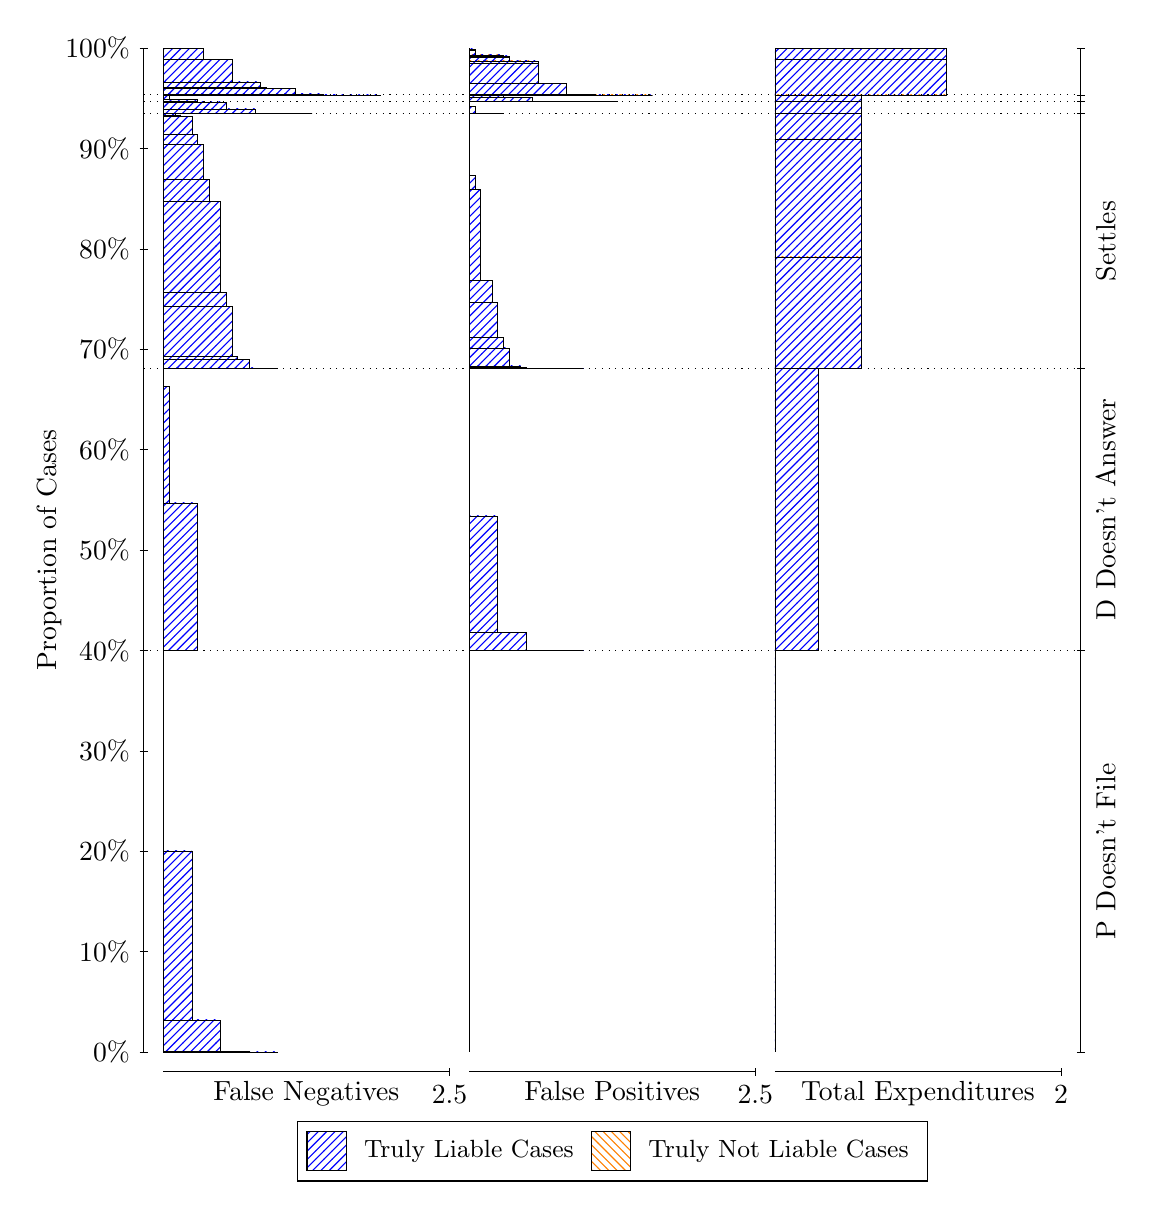
\begin{tikzpicture}
\draw[black, very thin] (1.5,1.75) -- (1.5,14.5);
\node[rotate=90, text=black, anchor=center] at (0.3, 8.125) {Proportion of Cases};
\draw[black, very thin] (1.45,1.75) -- (1.55,1.75);
\node[text=black, anchor=east] at (1.45, 1.75) {0\%};
\draw[black, very thin] (1.45,3.025) -- (1.55,3.025);
\node[text=black, anchor=east] at (1.45, 3.025) {10\%};
\draw[black, very thin] (1.45,4.3) -- (1.55,4.3);
\node[text=black, anchor=east] at (1.45, 4.3) {20\%};
\draw[black, very thin] (1.45,5.575) -- (1.55,5.575);
\node[text=black, anchor=east] at (1.45, 5.575) {30\%};
\draw[black, very thin] (1.45,6.85) -- (1.55,6.85);
\node[text=black, anchor=east] at (1.45, 6.85) {40\%};
\draw[black, very thin] (1.45,8.125) -- (1.55,8.125);
\node[text=black, anchor=east] at (1.45, 8.125) {50\%};
\draw[black, very thin] (1.45,9.4) -- (1.55,9.4);
\node[text=black, anchor=east] at (1.45, 9.4) {60\%};
\draw[black, very thin] (1.45,10.675) -- (1.55,10.675);
\node[text=black, anchor=east] at (1.45, 10.675) {70\%};
\draw[black, very thin] (1.45,11.95) -- (1.55,11.95);
\node[text=black, anchor=east] at (1.45, 11.95) {80\%};
\draw[black, very thin] (1.45,13.225) -- (1.55,13.225);
\node[text=black, anchor=east] at (1.45, 13.225) {90\%};
\draw[black, very thin] (1.45,14.5) -- (1.55,14.5);
\node[text=black, anchor=east] at (1.45, 14.5) {100\%};

\draw[black, very thin] (13.4,1.75) -- (13.4,14.5);
\draw[black, very thin] (13.35,1.75) -- (13.45,1.75);
\node[anchor=west] at (13.35, 1.75) {};
\draw[black, very thin] (13.35,6.8489) -- (13.45,6.8489);
\node[anchor=west] at (13.35, 6.8489) {};
\draw[black, very thin] (13.35,10.432) -- (13.45,10.432);
\node[anchor=west] at (13.35, 10.432) {};
\draw[black, very thin] (13.35,13.668) -- (13.45,13.668);
\node[anchor=west] at (13.35, 13.668) {};
\draw[black, very thin] (13.35,13.819) -- (13.45,13.819);
\node[anchor=west] at (13.35, 13.819) {};
\draw[black, very thin] (13.35,13.906) -- (13.45,13.906);
\node[anchor=west] at (13.35, 13.906) {};
\draw[black, very thin] (13.35,14.5) -- (13.45,14.5);
\node[anchor=west] at (13.35, 14.5) {};

\draw[black, very thin, pattern color=blue, pattern=north east lines] (1.75,1.75) rectangle (3.2033,1.75);
\draw[black, very thin, pattern color=blue, pattern=north east lines] (1.75,1.75) rectangle (2.84,1.7534);
\draw[black, very thin, pattern color=blue, pattern=north east lines] (1.75,1.7534) rectangle (2.4767,2.158);
\draw[black, very thin, pattern color=blue, pattern=north east lines] (1.75,2.158) rectangle (2.1133,4.3029);
\draw[black, very thin, pattern color=orange, pattern=north west lines] (1.75,4.3029) rectangle (1.75,4.3029);
\draw[black, very thin, pattern color=blue, pattern=north east lines] (1.75,4.3029) rectangle (1.75,6.8489);
\draw[black, very thin, pattern color=blue, pattern=north east lines] (1.75,6.8489) rectangle (2.186,8.723);
\draw[black, very thin, pattern color=blue, pattern=north east lines] (1.75,8.723) rectangle (1.8227,10.201);
\draw[black, very thin, pattern color=orange, pattern=north west lines] (1.75,10.201) rectangle (1.75,10.201);
\draw[black, very thin, pattern color=blue, pattern=north east lines] (1.75,10.201) rectangle (1.75,10.432);
\draw[black, very thin, pattern color=blue, pattern=north east lines] (1.75,10.432) rectangle (3.2033,10.432);
\draw[black, very thin, pattern color=blue, pattern=north east lines] (1.75,10.432) rectangle (3.058,10.432);
\draw[black, very thin, pattern color=blue, pattern=north east lines] (1.75,10.432) rectangle (2.9127,10.437);
\draw[black, very thin, pattern color=blue, pattern=north east lines] (1.75,10.437) rectangle (2.84,10.55);
\draw[black, very thin, pattern color=blue, pattern=north east lines] (1.75,10.55) rectangle (2.6947,10.58);
\draw[black, very thin, pattern color=blue, pattern=north east lines] (1.75,10.58) rectangle (2.622,11.216);
\draw[black, very thin, pattern color=blue, pattern=north east lines] (1.75,11.216) rectangle (2.5493,11.393);
\draw[black, very thin, pattern color=blue, pattern=north east lines] (1.75,11.393) rectangle (2.4767,12.55);
\draw[black, very thin, pattern color=blue, pattern=north east lines] (1.75,12.55) rectangle (2.3313,12.827);
\draw[black, very thin, pattern color=blue, pattern=north east lines] (1.75,12.827) rectangle (2.2587,13.278);
\draw[black, very thin, pattern color=blue, pattern=north east lines] (1.75,13.278) rectangle (2.186,13.408);
\draw[black, very thin, pattern color=blue, pattern=north east lines] (1.75,13.408) rectangle (2.1133,13.636);
\draw[black, very thin, pattern color=blue, pattern=north east lines] (1.75,13.636) rectangle (1.968,13.65);
\draw[black, very thin, pattern color=blue, pattern=north east lines] (1.75,13.65) rectangle (1.8953,13.666);
\draw[black, very thin, pattern color=blue, pattern=north east lines] (1.75,13.666) rectangle (1.8227,13.667);
\draw[black, very thin, pattern color=orange, pattern=north west lines] (1.75,13.667) rectangle (1.75,13.667);
\draw[black, very thin, pattern color=blue, pattern=north east lines] (1.75,13.667) rectangle (1.75,13.668);
\draw[black, very thin, pattern color=blue, pattern=north east lines] (1.75,13.668) rectangle (3.6393,13.668);
\draw[black, very thin, pattern color=blue, pattern=north east lines] (1.75,13.668) rectangle (3.276,13.668);
\draw[black, very thin, pattern color=blue, pattern=north east lines] (1.75,13.668) rectangle (2.9127,13.726);
\draw[black, very thin, pattern color=blue, pattern=north east lines] (1.75,13.726) rectangle (2.5493,13.817);
\draw[black, very thin, pattern color=blue, pattern=north east lines] (1.75,13.817) rectangle (2.186,13.819);
\draw[black, very thin, pattern color=orange, pattern=north west lines] (1.75,13.819) rectangle (1.75,13.819);
\draw[black, very thin, pattern color=blue, pattern=north east lines] (1.75,13.819) rectangle (2.186,13.85);
\draw[black, very thin, pattern color=blue, pattern=north east lines] (1.75,13.85) rectangle (1.8227,13.904);
\draw[black, very thin, pattern color=orange, pattern=north west lines] (1.75,13.904) rectangle (1.75,13.904);
\draw[black, very thin, pattern color=blue, pattern=north east lines] (1.75,13.904) rectangle (1.75,13.906);
\draw[black, very thin, pattern color=blue, pattern=north east lines] (1.75,13.906) rectangle (4.5113,13.906);
\draw[black, very thin, pattern color=blue, pattern=north east lines] (1.75,13.906) rectangle (4.148,13.906);
\draw[black, very thin, pattern color=blue, pattern=north east lines] (1.75,13.906) rectangle (3.7847,13.918);
\draw[black, very thin, pattern color=blue, pattern=north east lines] (1.75,13.918) rectangle (3.712,13.918);
\draw[black, very thin, pattern color=blue, pattern=north east lines] (1.75,13.918) rectangle (3.4213,13.992);
\draw[black, very thin, pattern color=blue, pattern=north east lines] (1.75,13.992) rectangle (3.3487,13.992);
\draw[black, very thin, pattern color=blue, pattern=north east lines] (1.75,13.992) rectangle (3.058,14.005);
\draw[black, very thin, pattern color=blue, pattern=north east lines] (1.75,14.005) rectangle (2.9853,14.069);
\draw[black, very thin, pattern color=blue, pattern=north east lines] (1.75,14.069) rectangle (2.6947,14.069);
\draw[black, very thin, pattern color=blue, pattern=north east lines] (1.75,14.069) rectangle (2.622,14.355);
\draw[black, very thin, pattern color=blue, pattern=north east lines] (1.75,14.355) rectangle (2.3313,14.355);
\draw[black, very thin, pattern color=blue, pattern=north east lines] (1.75,14.355) rectangle (2.2587,14.492);
\draw[black, very thin, pattern color=blue, pattern=north east lines] (1.75,14.492) rectangle (1.8953,14.5);
\draw[black, very thin, pattern color=orange, pattern=north west lines] (1.75,14.5) rectangle (1.75,14.5);
\draw[black, very thin, pattern color=blue, pattern=north east lines] (1.75,14.5) rectangle (1.75,14.5);
\draw[black, very thin, pattern color=orange, pattern=north west lines] (5.6333,1.75) rectangle (5.6333,1.75);
\draw[black, very thin, pattern color=blue, pattern=north east lines] (5.6333,1.75) rectangle (5.6333,6.8489);
\draw[black, very thin, pattern color=orange, pattern=north west lines] (5.6333,6.8489) rectangle (7.0867,6.8489);
\draw[black, very thin, pattern color=blue, pattern=north east lines] (5.6333,6.8489) rectangle (7.0867,6.8489);
\draw[black, very thin, pattern color=blue, pattern=north east lines] (5.6333,6.8489) rectangle (6.7233,6.8492);
\draw[black, very thin, pattern color=blue, pattern=north east lines] (5.6333,6.8492) rectangle (6.36,7.0796);
\draw[black, very thin, pattern color=blue, pattern=north east lines] (5.6333,7.0796) rectangle (5.9967,8.5576);
\draw[black, very thin, pattern color=blue, pattern=north east lines] (5.6333,8.5576) rectangle (5.6333,10.432);
\draw[black, very thin, pattern color=orange, pattern=north west lines] (5.6333,10.432) rectangle (7.0867,10.432);
\draw[black, very thin, pattern color=blue, pattern=north east lines] (5.6333,10.432) rectangle (7.0867,10.432);
\draw[black, very thin, pattern color=orange, pattern=north west lines] (5.6333,10.432) rectangle (6.796,10.432);
\draw[black, very thin, pattern color=blue, pattern=north east lines] (5.6333,10.432) rectangle (6.796,10.432);
\draw[black, very thin, pattern color=blue, pattern=north east lines] (5.6333,10.432) rectangle (6.7233,10.432);
\draw[black, very thin, pattern color=orange, pattern=north west lines] (5.6333,10.432) rectangle (6.6507,10.432);
\draw[black, very thin, pattern color=blue, pattern=north east lines] (5.6333,10.432) rectangle (6.6507,10.432);
\draw[black, very thin, pattern color=orange, pattern=north west lines] (5.6333,10.432) rectangle (6.5053,10.432);
\draw[black, very thin, pattern color=blue, pattern=north east lines] (5.6333,10.432) rectangle (6.5053,10.432);
\draw[black, very thin, pattern color=blue, pattern=north east lines] (5.6333,10.432) rectangle (6.4327,10.433);
\draw[black, very thin, pattern color=blue, pattern=north east lines] (5.6333,10.433) rectangle (6.36,10.449);
\draw[black, very thin, pattern color=blue, pattern=north east lines] (5.6333,10.449) rectangle (6.2873,10.463);
\draw[black, very thin, pattern color=blue, pattern=north east lines] (5.6333,10.463) rectangle (6.142,10.691);
\draw[black, very thin, pattern color=blue, pattern=north east lines] (5.6333,10.691) rectangle (6.0693,10.822);
\draw[black, very thin, pattern color=blue, pattern=north east lines] (5.6333,10.822) rectangle (5.9967,11.273);
\draw[black, very thin, pattern color=blue, pattern=north east lines] (5.6333,11.273) rectangle (5.924,11.55);
\draw[black, very thin, pattern color=blue, pattern=north east lines] (5.6333,11.55) rectangle (5.7787,12.706);
\draw[black, very thin, pattern color=blue, pattern=north east lines] (5.6333,12.706) rectangle (5.706,12.884);
\draw[black, very thin, pattern color=blue, pattern=north east lines] (5.6333,12.884) rectangle (5.6333,13.668);
\draw[black, very thin, pattern color=orange, pattern=north west lines] (5.6333,13.668) rectangle (6.0693,13.668);
\draw[black, very thin, pattern color=blue, pattern=north east lines] (5.6333,13.668) rectangle (6.0693,13.67);
\draw[black, very thin, pattern color=blue, pattern=north east lines] (5.6333,13.67) rectangle (5.706,13.761);
\draw[black, very thin, pattern color=blue, pattern=north east lines] (5.6333,13.761) rectangle (5.6333,13.819);
\draw[black, very thin, pattern color=orange, pattern=north west lines] (5.6333,13.819) rectangle (7.5227,13.819);
\draw[black, very thin, pattern color=blue, pattern=north east lines] (5.6333,13.819) rectangle (7.5227,13.819);
\draw[black, very thin, pattern color=blue, pattern=north east lines] (5.6333,13.819) rectangle (7.1593,13.819);
\draw[black, very thin, pattern color=blue, pattern=north east lines] (5.6333,13.819) rectangle (6.796,13.821);
\draw[black, very thin, pattern color=blue, pattern=north east lines] (5.6333,13.821) rectangle (6.4327,13.875);
\draw[black, very thin, pattern color=blue, pattern=north east lines] (5.6333,13.875) rectangle (6.0693,13.906);
\draw[black, very thin, pattern color=orange, pattern=north west lines] (5.6333,13.906) rectangle (7.9587,13.906);
\draw[black, very thin, pattern color=blue, pattern=north east lines] (5.6333,13.906) rectangle (7.9587,13.906);
\draw[black, very thin, pattern color=orange, pattern=north west lines] (5.6333,13.906) rectangle (7.5953,13.906);
\draw[black, very thin, pattern color=blue, pattern=north east lines] (5.6333,13.906) rectangle (7.5953,13.906);
\draw[black, very thin, pattern color=orange, pattern=north west lines] (5.6333,13.906) rectangle (7.232,13.906);
\draw[black, very thin, pattern color=blue, pattern=north east lines] (5.6333,13.906) rectangle (7.232,13.914);
\draw[black, very thin, pattern color=blue, pattern=north east lines] (5.6333,13.914) rectangle (6.8687,14.051);
\draw[black, very thin, pattern color=orange, pattern=north west lines] (5.6333,14.051) rectangle (6.8687,14.051);
\draw[black, very thin, pattern color=blue, pattern=north east lines] (5.6333,14.051) rectangle (6.8687,14.051);
\draw[black, very thin, pattern color=orange, pattern=north west lines] (5.6333,14.051) rectangle (6.796,14.051);
\draw[black, very thin, pattern color=blue, pattern=north east lines] (5.6333,14.051) rectangle (6.796,14.051);
\draw[black, very thin, pattern color=blue, pattern=north east lines] (5.6333,14.051) rectangle (6.5053,14.302);
\draw[black, very thin, pattern color=blue, pattern=north east lines] (5.6333,14.302) rectangle (6.5053,14.337);
\draw[black, very thin, pattern color=orange, pattern=north west lines] (5.6333,14.337) rectangle (6.4327,14.337);
\draw[black, very thin, pattern color=blue, pattern=north east lines] (5.6333,14.337) rectangle (6.4327,14.337);
\draw[black, very thin, pattern color=blue, pattern=north east lines] (5.6333,14.337) rectangle (6.142,14.387);
\draw[black, very thin, pattern color=blue, pattern=north east lines] (5.6333,14.387) rectangle (6.142,14.401);
\draw[black, very thin, pattern color=blue, pattern=north east lines] (5.6333,14.401) rectangle (6.0693,14.413);
\draw[black, very thin, pattern color=orange, pattern=north west lines] (5.6333,14.413) rectangle (6.0693,14.413);
\draw[black, very thin, pattern color=blue, pattern=north east lines] (5.6333,14.413) rectangle (6.0693,14.414);
\draw[black, very thin, pattern color=blue, pattern=north east lines] (5.6333,14.414) rectangle (5.7787,14.414);
\draw[black, very thin, pattern color=blue, pattern=north east lines] (5.6333,14.414) rectangle (5.7787,14.414);
\draw[black, very thin, pattern color=blue, pattern=north east lines] (5.6333,14.414) rectangle (5.706,14.472);
\draw[black, very thin, pattern color=blue, pattern=north east lines] (5.6333,14.472) rectangle (5.706,14.488);
\draw[black, very thin, pattern color=blue, pattern=north east lines] (5.6333,14.488) rectangle (5.6333,14.5);
\draw[black, very thin, pattern color=orange, pattern=north west lines] (9.5167,1.75) rectangle (9.5167,1.75);
\draw[black, very thin, pattern color=blue, pattern=north east lines] (9.5167,1.75) rectangle (9.5167,6.8489);
\draw[black, very thin, pattern color=orange, pattern=north west lines] (9.5167,6.8489) rectangle (10.062,6.8489);
\draw[black, very thin, pattern color=blue, pattern=north east lines] (9.5167,6.8489) rectangle (10.062,10.432);
\draw[black, very thin, pattern color=orange, pattern=north west lines] (9.5167,10.432) rectangle (10.607,10.432);
\draw[black, very thin, pattern color=blue, pattern=north east lines] (9.5167,10.432) rectangle (10.607,11.848);
\draw[black, very thin, pattern color=orange, pattern=north west lines] (9.5167,11.848) rectangle (10.607,11.848);
\draw[black, very thin, pattern color=blue, pattern=north east lines] (9.5167,11.848) rectangle (10.607,13.346);
\draw[black, very thin, pattern color=orange, pattern=north west lines] (9.5167,13.346) rectangle (10.607,13.346);
\draw[black, very thin, pattern color=blue, pattern=north east lines] (9.5167,13.346) rectangle (10.607,13.668);
\draw[black, very thin, pattern color=orange, pattern=north west lines] (9.5167,13.668) rectangle (10.607,13.668);
\draw[black, very thin, pattern color=blue, pattern=north east lines] (9.5167,13.668) rectangle (10.607,13.819);
\draw[black, very thin, pattern color=orange, pattern=north west lines] (9.5167,13.819) rectangle (10.607,13.819);
\draw[black, very thin, pattern color=blue, pattern=north east lines] (9.5167,13.819) rectangle (10.607,13.906);
\draw[black, very thin, pattern color=orange, pattern=north west lines] (9.5167,13.906) rectangle (11.697,13.906);
\draw[black, very thin, pattern color=blue, pattern=north east lines] (9.5167,13.906) rectangle (11.697,14.351);
\draw[black, very thin, pattern color=orange, pattern=north west lines] (9.5167,14.351) rectangle (11.697,14.351);
\draw[black, very thin, pattern color=blue, pattern=north east lines] (9.5167,14.351) rectangle (11.697,14.5);
\draw[black, dotted] (1.5,6.8489) -- (13.4,6.8489);
\draw[black, dotted] (1.5,10.432) -- (13.4,10.432);
\draw[black, dotted] (1.5,13.668) -- (13.4,13.668);
\draw[black, dotted] (1.5,13.819) -- (13.4,13.819);
\draw[black, dotted] (1.5,13.906) -- (13.4,13.906);
\draw[black, very thin] (1.75,1.5) -- (5.3833,1.5);
\node[text=black, anchor=north] at (3.5667, 1.5) {False Negatives};
\draw[black, very thin] (5.3833,1.45) -- (5.3833,1.55);
\node[text=black, anchor=north] at (5.3833, 1.45) {2.5};

\draw[black, very thin] (5.6333,1.5) -- (9.2667,1.5);
\node[text=black, anchor=north] at (7.45, 1.5) {False Positives};
\draw[black, very thin] (9.2667,1.45) -- (9.2667,1.55);
\node[text=black, anchor=north] at (9.2667, 1.45) {2.5};

\draw[black, very thin] (9.5167,1.5) -- (13.15,1.5);
\node[text=black, anchor=north] at (11.333, 1.5) {Total Expenditures};
\draw[black, very thin] (13.15,1.45) -- (13.15,1.55);
\node[text=black, anchor=north] at (13.15, 1.45) {2};

\node[text=black, centered, rotate=90] at (13.72, 4.2994) {P Doesn't File};
\node[text=black, centered, rotate=90] at (13.72, 8.6403) {D Doesn't Answer};
\node[text=black, centered, rotate=90] at (13.72, 12.05) {Settles};




\draw (7.449999999999999,1.5) node[draw=none] (baseCoordinate) {};
\begin{scope}[align=center]
        \matrix[scale=0.5, draw=black, below=0.5cm of baseCoordinate, nodes={draw}, column sep=0.1cm]{
            \node[rectangle, draw, minimum width=0.5cm, minimum height=0.5cm, pattern color=blue, pattern=north east lines] {}; &
            \node[draw=none, font=\small, text=black] (B) {Truly Liable Cases}; &
            \node[rectangle, draw, minimum width=0.5cm, minimum height=0.5cm, pattern color=orange, pattern=north west lines] {}; &
            \node[draw=none, font=\small, text=black] (B) {Truly Not Liable Cases}; \\
            };
\end{scope}

\end{tikzpicture}
\end{document}